\subsection{An exchange-grid algorithm for portfolio certificates}
\label{sec:exchange_grid}

The portfolio objective in Equation~\eqref{eq:ellipsoid} is a mean-risk
combinatorial problem under ellipsoidal uncertainty. Ellipsoidal ambiguity,
branch-and-bound for mean-risk problems and approximate trade-off sets are
established approaches
\citep{kurtz2018,buchheim2018,papadimitriouyannakakis2000}. We study a different
computational representation for this specific reference-relative problem.
The proposed step is to carry coordinatewise rounding-residual bounds through
two signed subset-sum recurrences and join the resulting states by their
exchange count. The algorithm then uses the portfolio responsible for the
largest upper bound to adjust for risk directions omitted from the grid.
Each completed pass gives a feasible portfolio and an upper bound for the
original objective.

\subsubsection{Signed states and a residual certificate}

Write $a_i$ for row $i$ of $L$, viewed as a column, and let $P$ have orthonormal
columns spanning the risk directions represented in the grid. Choose a common
coordinate origin $o$ and positive steps $h$. Write each projected loading as
\[
 P^\top a_i=o+h\odot g_i+e_i,\qquad
 g_i=\mathrm{round}\!\left((P^\top a_i-o)\oslash h\right),
\]
where $\odot$ and $\oslash$ denote componentwise multiplication and division.
An assignment relative to the reference has $m$ additions and $m$ removals.
The $m$ copies of the origin contributed by the additions cancel the $m$ copies
contributed by the removals.

For each side separately, a subset-sum recurrence indexes its states by
$(m,g)$, where $g$ is the sum of signed keys. A state stores the maximum signed
nominal reward, a feasible subset attaining it, and coordinatewise minima and
maxima of the sum of signed residuals over all its subsets. Skipping an item
leaves its state unchanged. Taking the item shifts the count, the key and both
residual limits by the item's signed contributions. When two paths enter the
same state, the recurrence takes the larger reward and merges the residual
extrema. These extrema describe all reachable residuals coordinatewise.
The box may include residual combinations that no subset attains.

Join an addition cell and a removal cell with the same exchange count. Let
$M_+$ and $M_-$ be their maximum rewards, and let $R$ be their combined
residual box shifted by $h\odot(g_++g_-)$. The projected loading of every
portfolio in this join lies in $R$, so the join's upper bound is
\begin{equation}\label{eq:grid_bound}
 M_++M_- - r\,\operatorname{dist}_2(0,R).
\end{equation}
The maximum of \eqref{eq:grid_bound} across all joins and the reference is
an upper bound. Evaluating a joined pair of witnesses in the full objective
gives a feasible lower bound. A pass that stops before finishing its states
or joins contributes no upper bound. Earlier completed passes remain valid.

\begin{figure}[htbp]
\centering
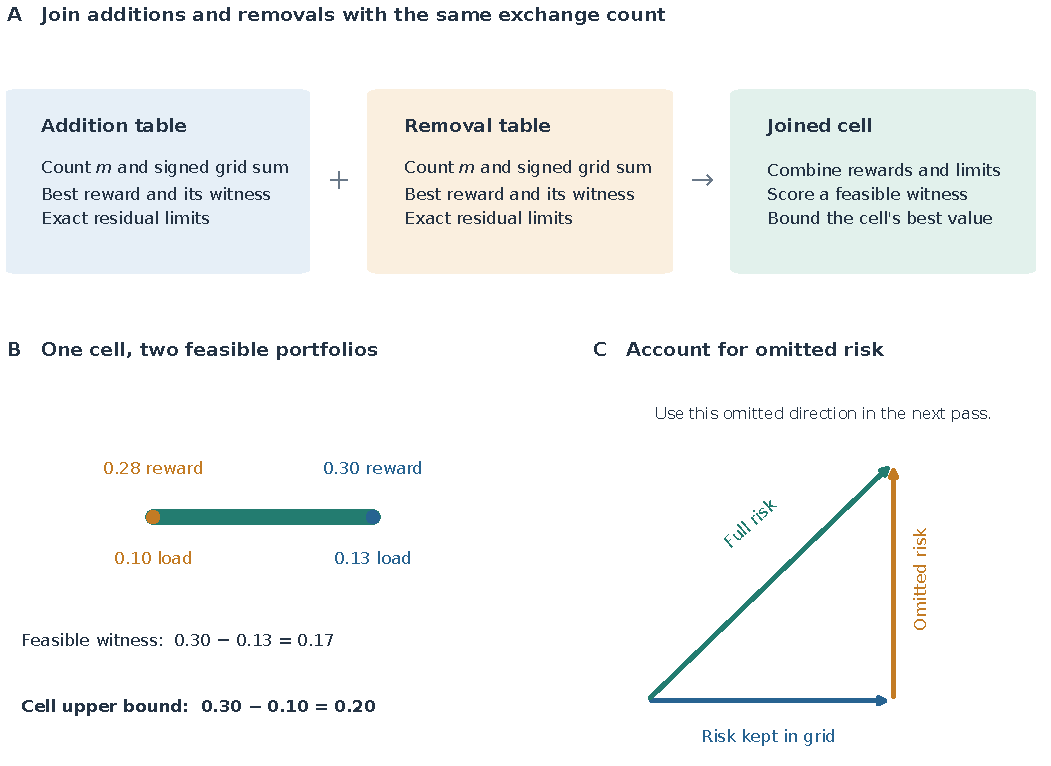
\includegraphics[width=\linewidth]{exchange_grid_algorithm.pdf}
\caption{Exchange-grid algorithm. Panel A shows how addition and removal states are joined. Panel B uses two illustrative portfolios to show how the cell bound is computed. Panel C decomposes the witness's load into the grid projection and the omitted component used to update the next pass.}
\label{fig:grid_algorithm}
\end{figure}

\paragraph{Numerical example.} Panel B of Figure~\ref{fig:grid_algorithm} illustrates how the certificate is constructed.
Suppose two portfolios fall in the same joined cell in a one-factor problem.
Their nominal gains are $0.30$ and $0.28$, and their exact signed risk loadings
are $0.13$ and $0.10$, respectively. With $r=1$, the nominal-gain witness
has objective $0.30-0.13=0.17$. The interval of exact loadings
$[0.10,0.13]$ gives an upper bound of $0.30-0.10=0.20$ for the cell.
The second portfolio actually achieves $0.18$. The bound is valid even
though the highest nominal gain and the smallest risk penalty come from
different portfolios. The solver can retain the first portfolio and the
interval, then use $[0.17,0.20]$ to bound the best objective in the cell.

\paragraph{Additive error and the lattice case.}
If the grid spans all risk directions, the portfolio formed from the two
reward-maximising witnesses in a join has exactly the reward used in
\eqref{eq:grid_bound}. Each coordinate of an item residual lies in an interval of
width $h_j$. The joined box for $m$ exchanges therefore has diameter at most
$2m\|h\|_2$. The norm is 1-Lipschitz, so the gap between \eqref{eq:grid_bound}
and this witness's true objective is at most $2mr\|h\|_2$. Applying this to
a maximising join proves the same additive error bound with
$m\leq\min(q,n-q)$. If the projected loadings lie on the grid, all residuals
vanish. A single count-and-loading recurrence over selected countries then
solves the projected problem exactly. The reference loading is subtracted
at the end. If this grid spans all risk directions, the solution is exact
for the full objective as well.

\subsubsection{Tilting the certificate towards omitted risk}

For a vector $v$ orthogonal to the grid span with $\|v\|_2\leq1$, every portfolio
loading $z=L^\top d$ satisfies
\[
 \|z\|_2 \;\geq\;
    v^\top z+\sqrt{1-\|v\|_2^2}\,\|P^\top z\|_2 .
\]
The right-hand side is the inner product of $z$ with a vector of norm at most
one, obtained by combining $v$ and the unit vector in the direction of its
projection. We can therefore run the same recurrence with the linear rewards
$\mu_i-r a_i^\top v$ and projected radius $r\sqrt{1-\|v\|_2^2}$. Its upper
bound remains valid for the full problem. We set the next tilt to
$(I-PP^\top)z_w/\|z_w\|_2$ using a witness from the preceding maximising join.
The norm inequality is then tight at that witness. The next pass can expose
a different portfolio whose bound is larger. Taking the smallest upper bound
from completed passes and the largest feasible lower bound keeps the certificate
valid. The lower bound always uses full risk, including dimensions omitted
from the grid.

\paragraph{Algorithm.}
Start with zero tilt. Evaluate the exposure reference and the portfolio with
the best nominal gain to initialise the lower bound. The best nominal gain
also gives an upper bound. At each grid resolution:
\begin{enumerate}
 \item Build the two signed tables and join states with the same exchange count.
 \item Find the join with the largest bound in \eqref{eq:grid_bound}, using the
       current adjusted rewards and projected radius. Evaluate its witness
       and any other promising witnesses with full risk.
 \item Keep the best feasible value and the smallest valid upper bound seen
       so far. Stop if their difference meets the tolerance. Otherwise update
       the tilt using the highest-bound join's witness and refine the grid.
\end{enumerate}
If a resource limit interrupts a pass, return the best feasible portfolio
and the bounds from completed passes.

The method has a computational trade-off. For fixed grid dimension, the number
of states grows polynomially in the exchange count and the grid resolution.
Fine or high-dimensional grids can be expensive. The implementation projects
onto at most two directions. It uses a dense recurrence when the projected
loadings lie on a small lattice and otherwise uses sparse signed states.
The early stopping certificate reports the cost of that compression in the
units of the original objective.

\subsubsection{Comparison on discrete and continuous inputs}

We compare against the integer cutting-plane method in
Section~\ref{sec:ellipsoid}. We also disable the tilt as a control. The benchmark
uses 16 instances per synthetic design and reconstructs the fitted objective
for each of the 12 agricultural holdout batches. Timing starts after the
benefits and factor loadings are supplied. The lattice designs give each
factor seven equally spaced levels. The continuous design uses six normally
distributed factor loadings per country. The gap tolerance is $10^{-5}$ in
total-gain units.
